\begin{exsol}{13}{Tadelis Exercise 8.8}{171--172}{Foundations}{L3}
\asked Set up the game tree of the entry story (NSG enters or not, then S\&P fights or
accommodates) and find the subgame-perfect equilibrium outcome.

\method Backward induction in a finite game of perfect information (Tadelis \S8.1,
Def.~8.1 and Prop.~8.1, pp.~151--153). With perfect information the subgame-perfect equilibria
are exactly the profiles that survive backward induction (Tadelis \S8.2, p.~158). Same structure
as the entry game of Cabral \S7.2 (\texttt{Notas/L03/L03-06}).

\solution
\textbf{Notation.} Players: NSG (the entrant, E) and S\&P (the incumbent, I). E chooses
$\mathit{In}$ or $\mathit{Out}$; after $\mathit{In}$, I chooses $W$ (price war) or $A$
(accommodate). Payoffs $(u_E, u_I)$ in \$ million of net present value. The entry cost of 2 is
sunk once E enters, so it is subtracted from every payoff that follows $\mathit{In}$:
\begin{align*}
  (u_E,u_I)(\mathit{Out}) &= (0,\ 10),\\
  (u_E,u_I)(\mathit{In},W) &= (1-2,\ 1) = (-1,\ 1),\\
  (u_E,u_I)(\mathit{In},A) &= (4-2,\ 4) = (2,\ 4).
\end{align*}
\begin{center}
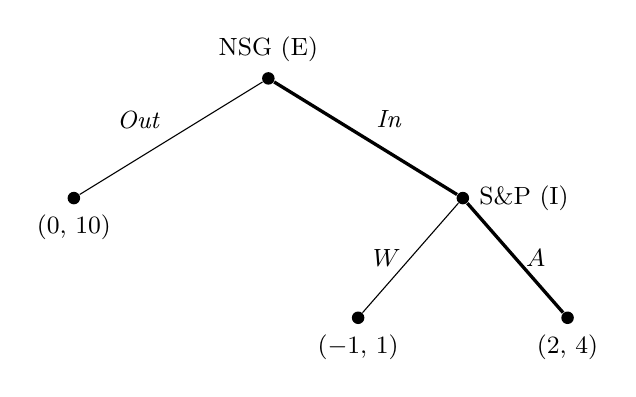
\begin{tikzpicture}[scale=0.95,dot/.style={circle,fill,inner sep=1.6pt},
  every node/.style={font=\small}]
  \node[dot,label=above:{NSG (E)}] (r) at (0,0) {};
  \node[dot,label=below:{$(0,\,10)$}] (o) at (-2.6,-1.6) {};
  \node[dot,label=right:{S\&P (I)}] (i) at (2.6,-1.6) {};
  \node[dot,label=below:{$(-1,\,1)$}] (w) at (1.2,-3.2) {};
  \node[dot,label=below:{$(2,\,4)$}] (a) at (4.0,-3.2) {};
  \draw (r) -- node[above left] {$\mathit{Out}$} (o);
  \draw[very thick] (r) -- node[above right] {$\mathit{In}$} (i);
  \draw (i) -- node[left] {$W$} (w);
  \draw[very thick] (i) -- node[right] {$A$} (a);
\end{tikzpicture}\\[2pt]
{\footnotesize Payoffs $(u_E, u_I)$; thick branches = backward-induction choices.}
\end{center}

\textbf{Step 1: the incumbent's node.} After entry, S\&P compares
\[
  u_I(\mathit{In},A) = 4 > 1 = u_I(\mathit{In},W),
\]
so it accommodates. The price war is not a credible response.

\textbf{Step 2: the entrant's node.} Replacing S\&P's node by its outcome $(2,4)$, NSG compares
\[
  u_E(\mathit{In}) = 2 > 0 = u_E(\mathit{Out}),
\]
so it enters.

\textbf{Step 3: the non-credible Nash equilibrium.} In the normal form (rows: E's strategies;
columns: I's strategies)
\begin{center}
\begin{tabular}{r|c|c|}
\multicolumn{1}{r}{} & \multicolumn{1}{c}{$W$} & \multicolumn{1}{c}{$A$}\\ \cline{2-3}
$\mathit{Out}$ & $0,\ 10$ & $0,\ 10$ \\ \cline{2-3}
$\mathit{In}$ & $-1,\ 1$ & $2,\ 4$ \\ \cline{2-3}
\end{tabular}
\end{center}
there are two pure Nash equilibria, $(\mathit{In},A)$ and $(\mathit{Out},W)$. In
$(\mathit{Out},W)$ the war is never fought, so the threat costs S\&P nothing; it fails
sequential rationality at the node S\&P never reaches (Tadelis Def.~7.8, p.~146; \S8.1).

\interp S\&P's prediction of a price war is cheap talk: once NSG has sunk its \$2 million, a war
gives S\&P 1 instead of 4, and NSG knows it. The incumbent would have to change its own payoffs
(capacity, a contract, a bond) to make the war credible, as in Cabral \S7.2.
The outcome does not depend on how the entry cost is booked: if ``each firm earns \$1 million''
were already net of it, NSG would still enter ($2 > 0$, and even a war would pay $1 > 0$).

\verify \texttt{check\_B\_L03.py} recomputes both backward-induction steps and the two pure
Nash equilibria of the $2\times2$ normal form. Tadelis prints no answer.

\answer{Tree above. Subgame-perfect equilibrium: NSG plays $\mathit{In}$, S\&P plays $A$
(accommodate); outcome: entry and accommodation, payoffs $(2, 4)$ in \$ million (NSG net of the
entry cost). $(\mathit{Out}, W)$ is a Nash equilibrium supported by a non-credible threat.}
\end{exsol}
